%!TEX root = ../dissertation.tex
\section[Blood Compartments of Cholinergic Systems and Small RNA Species]{Blood Compartments of Cholinergic Systems \\and Small RNA Species} \label{sec:stroke:celltypes}
To address the shortcomings of whole-blood RNA sequencing, which is more representative of the clinical setting, but less specific regarding cellular compartments, we consulted third party datasets to assess RNA species distribution in different cellular and non-cellular compartments of the blood. For small RNA species, we re-analysed a published dataset of small \ac{seq} of 450 human samples from various blood tissues;\cite{Juzenas2017} for large RNA transcripts, we utilised the tissue specificity of Marbach's regulatory circuits.\cite{Marbach2016} The large RNA information was used to identify blood cell types with cholinergic transcriptional activity, which was then used to zoom in into small RNA expression subsets related to cholinergic processes.

\begin{method}

\subsection{Large RNA Regulatory Circuits in Tissues of the Blood}
To evaluate the cell type distribution of cholinergic genes in blood tissue types, we utilised the expression patterns derived from cumulative transcription factor activity of Marbach's regulatory circuits.\cite{Marbach2016} As shown by the authors, the cumulative activity of all transcription factors towards one gene describe well the actual expression of that gene in the respective tissue type. To maximise comparability to the parallel analyses of small RNA species (Section \ref{sec:stroke:juzenas}), blood cell types (i.e., »regulatory circuits«) were selected to reflect the cell type selection of Juzenas \emph{et al.}\cite{Juzenas2017} based on similar markers of the »cluster of differentiation« family of genes. These were: CD4$^+$ T-helper cells, CD8$^+$ cytotoxic T-cells, CD14$^+$ monocytes, CD15$^+$ neutrophils, CD19$^+$ B-cells, CD56$^+$ natural killer cells, and, for comparison, whole blood. For the sake of simplicity, genes were considered »present« in each blood tissue type if at least one TF showed significant activity towards the gene.

TF activities were collected for all of the tissues and aggregated across all TFs per gene by summing. The resulting table of 15\,032 genes in the seven tissues was used as input for the \emph{Rtsne} function.\cite{Krijthe2015} t-SNE was computed using a range of perplexities and visualised as 2D map with a perplexity of 49 using R/ggplot2.\cite{Wickham2016}

\subsection{An Atlas of Small RNA Expression in Cell Types of the Blood} \label{sec:stroke:juzenas}
To evaluate the cell type distribution of our small RNA molecules, we analysed a dataset deposited by Juzenas \emph{et al.},\cite{Juzenas2017} who separated and sequenced 450 samples comprising seven types of individual blood cell types (characterised by »cluster of differentiation«-type membrane-bound receptors), serum, exosomes, and whole blood. The individual blood cell types comprised CD4$^+$ T-helper cells, CD8$^+$ cytotoxic T-cells, CD14$^+$ monocytes, CD15$^+$ neutrophils, CD19$^+$ B-cells, CD56$^+$ natural killer cells, and CD235a$^+$ erythrocytes (the only distinct cell type not available in Marbach's regulatory circuits, since mature erythrocytes do not transcribe). Starting from the raw data deposited on NCBI GEO, we controlled the quality, applied quality-based filtering, and aligned the 450 samples to miRNA and tRF sequences, as described in Section \ref{sec:stroke:alignment}. The original publication did not offer statistical analyses because of a failure in the spike-in procedure, and defined presence of a small RNA by a measure of at least five counts in 85\% of samples. However, since this definition relies heavily on sequencing depth, and depth can vary widely even in methodically robust sequencing experiments depending on a large number of variables (see Figure \ref{fig:read-quality-length}\,C), we defined our own test for descriptive analysis of presence or absence of lowly expressed small RNAs in each of the sample types (Section \ref{sec:stroke:presence}).

\subsection[Definition of Presence and Absence of Lowly Expressed\texorpdfstring{\\}{} smRNA Molecules]{Definition of Presence and Absence of Lowly Expressed smRNA Molecules} \label{sec:stroke:presence}
This definition comprises estimation of a log-normal distribution from a small RNA expression profile, and a statistical test to refute the null hypothesis that the distribution is in fact log-normal. The danger of evaluating true expression of lowly expressed smRNA molecules by a count-based threshold is the possibility of random reads resulting from degradation products of highly expressed RNA with similar sequence, and the amplification of noise. Both problems are exacerbated by an increase in sequencing depth. In today's \ac{seq} technology, most chips can accommodate only a limited amount of samples compared to the amount of reads that can be generated. While this is not as problematic in cases of longer inserts and paired design, which is usually employed in large \ac{seq}, in small \ac{seq} this can lead to enormous overheads of reads. It is not uncommon to receive tens of millions of reads for each sample, which exceeds the recommended amount (of at least one million) by large margins.

Thus, there is the need to distinguish between degradation products of highly expressed RNA molecules or amplified noise and legitimate lowly expressed smRNA molecules (even more so since one of the smRNA species is a product of non-random tRNA degradation). The central assumption for our proposed method is: The expression pattern of legitimate smRNA molecules follows, as is common in biology, a normal distribution of some kind, or, for the discrete case, a normal poisson distribution. On the other hand, degradation products or noise would rather follow other, »non-biological« distributions, such as a uniform distribution or a monotonously decreasing power-law distribution such as the Pareto distribution. Thus, we chose to statistically test each smRNA in each tissue type for the adherence to this criterion, by comparing the measured counts with a distribution function estimated based on the mean and standard deviation of the measured counts. During testing, we found the log-normal distribution to give the best classification results.
 
The distribution mean and standard deviation of the expression values per cell type and smRNA were estimated using the \emph{fitdist} function of the R/fitdistrplus package.\cite{Delignette-Muller2015} The count distribution was then tested against a log-normal distribution with the estimated mean and standard deviation via the R implementation of the Kolmogorov\=/Smirnov test, with a cutoff of 0.1. The small RNA was defined as present if the test failed to reject the null hypothesis (see Appendix \ref{appendix:presence-absence} for numerous examples).

\subsubsection{Analysis of Expression Patterns and Establishment of Virtual Tissues}
The distribution of smRNA expression across the different cell types was used to assign eight functional compartments (i.e., »virtual tissues«) to the entirety of detected fragments such that each smRNA was sorted into one of the tissue classes. Ideally, these classes would be unambiguous, i.e., there would be no overlap of smRNA molecules between the classes. Eight classes were created via hierarchical clustering of miRNA and tRF expression separately (Figure \ref{fig:heatmaps-small}), and then used in combination with t-SNE applied to the entire expression matrix, to visualise the compartmentalisation of smRNAs in these virtual tissues. The samples taken from stroke patients in the PREDICT study were sequenced from whole blood, which precludes direct information about tissue distribution. Thus, the two-dimensional maps from t-SNE visualisation were used to, first, explore the tissue association of smRNAs differentially expressed in whole blood samples of stroke patients, and second, examine the potential impact of \acl{ca} smRNAs in these tissues.

\end{method}

\begin{figure}
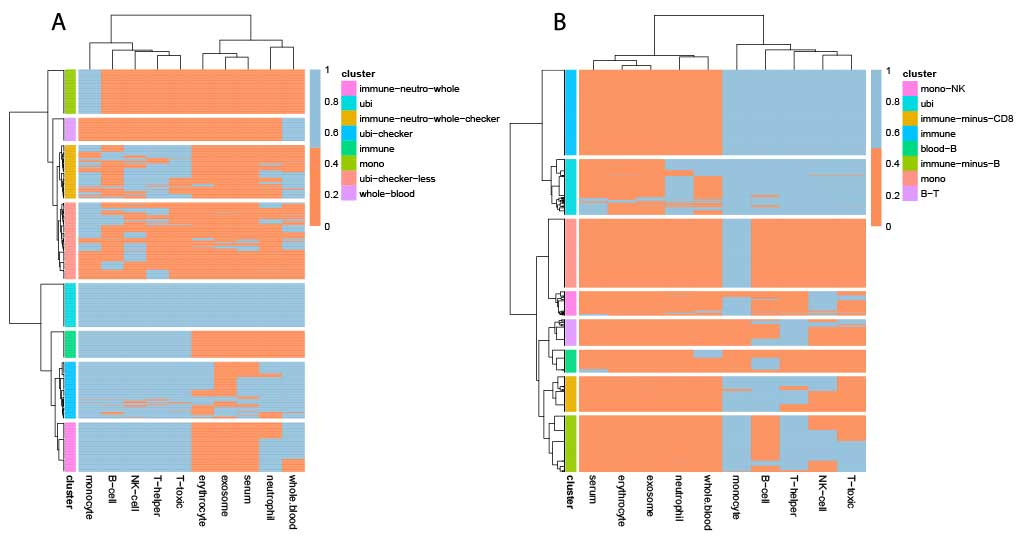
\includegraphics[width=\textwidth]{figures/heatmaps-small}
\caption[Functional Characterisation of Hierarchical Clusters in Blood Cell Small RNA Expression.]{\textbf{Functional Characterisation of Hierarchical Clusters in Blood Cell Small RNA Expression.} Information on presence/absence of miRNAs and tRFs in the tissue types analysed in Juzenas \emph{et al.}\cite{Juzenas2017} were hierarchically clustered into 8 clusters using the Ward method,\cite{Ward1963} and plotted on a heatmap (single smRNAs on the y-axis, tissue types on the x-axis). To assign meaning to these clusters, manual inspection was followed by annotation of enrichment in tissue types. Complex combinations were approximated by their most prominent features. \textbf{A)} Clusters of miRNA presence/absence in blood cell compartments. Clearest cluster association was shown by miRNAs expressed only in monocytes (»mono«), in all blood-borne immune cells except neutrophils (»immune«), ubiquitously without exception (»ubi«), and only in whole blood (i.e., in none of the single compartments (»whole-blood«). \textbf{B)} Clusters of tRF presence/absence in blood cell compartments. Clearest cluster association was shown by tRFs expressed only in monocytes (»mono«), and in all blood-borne immune cells except neutrophils (»immune«). The other tissue-related clusters were not as clear as in the miRNA expression data, indicating a looser association to cell type of tRNA-derived smRNAs.
\label{fig:heatmaps-small}}
\end{figure}

\subsection{Large RNA Expression Patterns Identify Cholinergic Systems\\ in CD14$^+$ Monocytes}
The expression patterns of 15\,032 large RNA molecules in blood-borne immune cells were visualised in a t-SNE-derived 2D map (Figure \ref{fig:tsne-large}\,A). More than half of all transcripts show highest expression in whole blood (7533, not shown), so subsequent analyses were performed on the set of six tissues, without the whole blood compartment. In this set (14\,280 genes), most transcripts show highest expression in CD14$^+$ monocytes (9125 transcripts), followed by CD19$^+$ B-cells (1176) and CD15$^+$ neutrophils (1166). Remaining are CD4$^+$ T-helper cells (1092), CD56$^+$ NK-cells (948), and CD8$^+$ cytotoxic T-cells (773). When filtered for cholinergic genes, there is visible enrichment of core cholinergic transcripts in a spatial sub-compartment of CD14$^+$ monocytes (Figure \ref{fig:tsne-large}\,B). Considering the different monocyte phenotypes (pro- and anti-inflam"-ma"-to"-ry, see Section \ref{sec:intro:stroke}), and their implied transcriptomic differences, which most likely are brought on by divergent TF activity, this compartmentalisation of cholinergic transcripts inside one spatial sub-compartment may indicate a cholinergic »preference« in favour of one particular monocyte phenotype. 

\begin{figure}[hb]
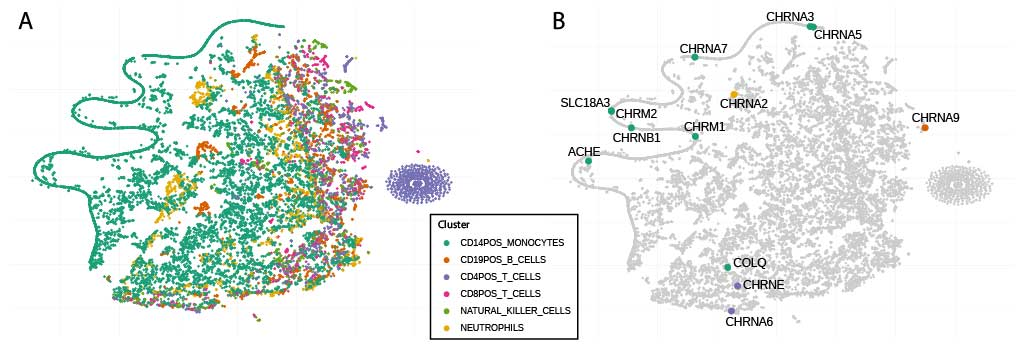
\includegraphics[width=\textwidth]{figures/tsne-large}
\caption[Large RNA Expression Patterns in Blood-Borne Cells.]{\textbf{Large RNA Expression Patterns in Blood-Borne Cells.} Expression derived from transcriptional activity in blood-borne cell types in the Marbach dataset\cite{Marbach2016} was visualised via t-SNE. The input matrix comprised all 14\,280 detected genes in 6 types of blood-borne immune cells. Genes were plotted on the first two t-SNE dimensions and coloured by the cell type of their highest expression, i.e., the highest cumulative transcriptional activity of all active TFs. \textbf{A)} Complete t-SNE shows a gradient of expression across the different cell types, with much expression in CD14$^+$ monocytes and T-cells. \textbf{B)} Highlighting of cholinergic core genes reveals an enrichment in close compartments of CD14$^+$ monocytes. The vesicular ACh-transporter SLC18A3 can serve as substitute for the main cholinergic marker, CHAT, as discussed in Section \ref{sec:database:tf}.
\label{fig:tsne-large}}
\end{figure}

\subsection{Identification of Functional Enrichment of \\smRNA Expression in Blood-Borne Cells}
To date, there is no comprehensive expression catalogue of smRNA species expression in the tissue types of the human body that is comparable to what has been achieved in the description of large RNA. To classify the detected smRNAs in a manner specific to tissues in human blood, we utilised a dataset published by Juzenas \emph{et al.},\cite{Juzenas2017} who describe miRNA expression in a variety of blood tissues. We re-analysed the publicly deposited data for miRNA and tRF expression, and developed our own method of defining »presence« of the smRNA in each tissue type based on the evaluation of a log-normal distribution model (instead of using a simple count threshold, see Section \ref{sec:stroke:juzenas} for details). 

Using these presence/absence data, we first utilised hierarchical clustering to establish »virtual tissues« that could be assigned to each smRNA (Figure \ref{fig:heatmaps-small}) for later evaluation in the stroke patient sequencing. Both miRNAs as well as tRFs showed a number of smRNAs clearly associated with several compartments, whereas other compartments and smRNAs were distributed in a more complex manner. The ten tissue types of the Juzenas \emph{et al.}\cite{Juzenas2017} study were equally parted into two five-tissue superclusters by the expression patterns of both smRNA species (Figures \ref{fig:heatmaps-small}\,A\&B, x-axis). These two clusters distinguish immune from non-immune compartments in the blood, but for one notable exception: while the »immune supercluster« comprises monocytes, T-cells, B-cells, and NK-cells, the »non-immune supercluster« contains neutrophils in addition to erythrocytes and the non-cellular tissues serum, exosomes, and whole blood. Notably, the neutrophil samples cluster closest to the whole blood compartment in both smRNA species.

Two distinct virtual tissues showed high consistency in both smRNA species: a virtual tissue containing only CD14$^+$ monocytes and another tissue comprising all studied cellular immune components except neutrophils (i.e., monocytes, B-cells, both types of T-cells, and NK-cells). miRNAs (Figure \ref{fig:heatmaps-small}\,A), in addition, yield clear clusters for miRNAs expressed in whole blood, and for miRNAs expressed ubiquitously without exception. In tRFs (Figure \ref{fig:heatmaps-small}\,B), the general picture is more complex, as the clusters are often mixed.

\subsection{Expression Patterns of Differentially Expressed and\\ Cholinergic-Associated smRNAs}
Similarly to the visualisation of large RNA molecules, the expression patterns of 600 miRNAs and 1671 tRFs in ten tissues of the blood were visualised in t-SNE-derived 2D maps (Figure \ref{fig:tsne-small}\,A\&B). In the initial visualisation, the forming of multiple clusters according to some virtual tissues can be observed, while other virtual tissues are visibly more dispersed. Clearest clusters are formed in both cases by ubiquitously expressed smRNAs (»ubi«), smRNAs expressed only in monocytes (»mono«), and smRNAs equally expressed in all immune-related blood-borne cells except for neutrophils (»immune«). Examination of DE smRNAs on this 2D map shows a further parallel between miRNAs and tRFs (Figure \ref{fig:tsne-small}\,C\&D): differential expression after stroke takes place in all compartments of the blood, and highest changes in transcript amount (as measured by count-change) are observed in ubiquitously expressed smRNAs. Similarly, \acf{ca} miRNAs and tRFs (Figure \ref{fig:tsne-small}\,E\&F) are observed in all compartments, but the most highly differentially regulated CA smRNAs are expressed in all blood compartments alike. Notably, whole blood does not play a role in DE miRNAs, which may indicate lower relative importance of non-cellular blood compartments in terms of classification. In other words, most smRNAs that are found in non-cellular compartments are found in the cellular compartments as well, making them irrelevant for classification (however, their biological function in these non-cellular compartments remains a matter of interest).

On the other hand, smRNAs that are ubiquitously expressed are also detected in differential expression with high frequency and perturbation (see Figure \ref{fig:tsne-small}\,C\&D). In addition to a putatively significant biological function of these smRNAs, this may also indicate a covariation of broadness of expression with detection in whole blood differential expression. Presenting an important limitation, this possibility cannot be assessed in the present data, because it requires a stratification of blood tissues prior to sequencing, for instance via fluorescence-assisted or magnetic-activated cell sorting (FACS/MACS). This issue is further discussed in Section \ref{sec:discussion:stroke-blood}.

\begin{figure}
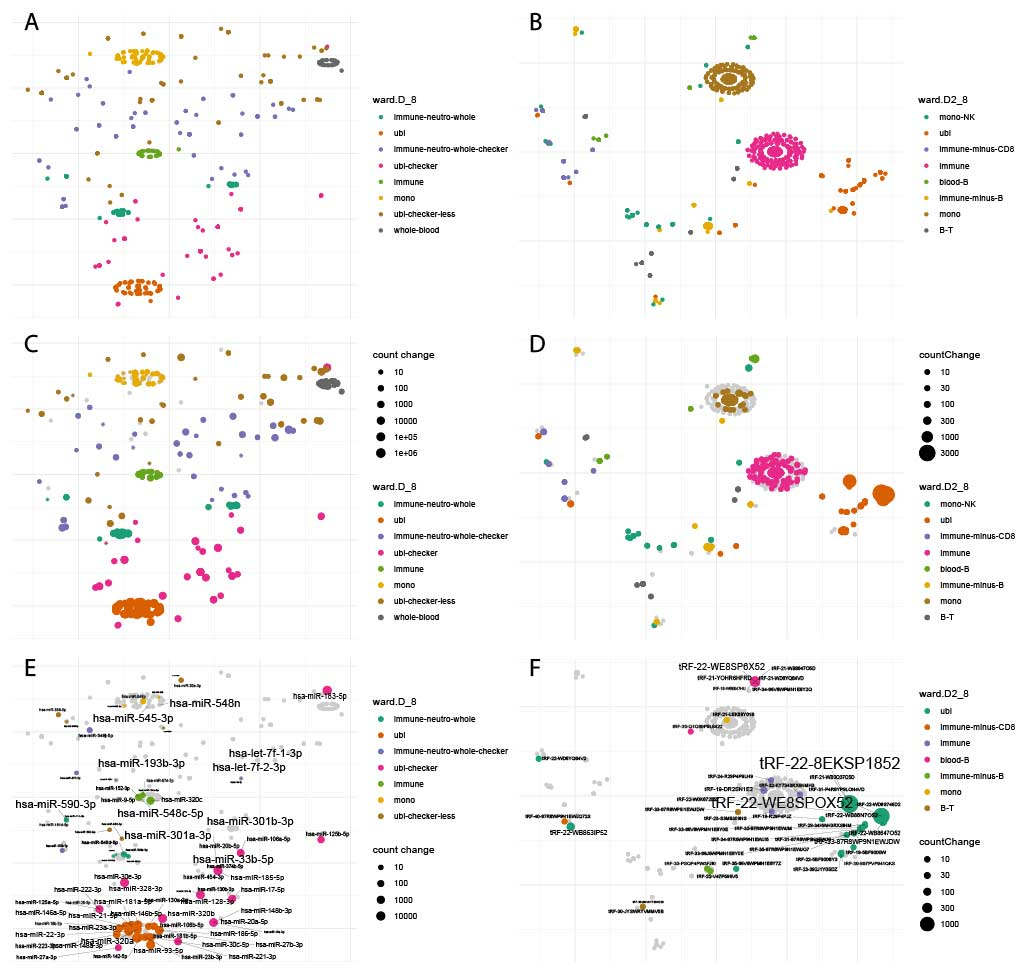
\includegraphics[width=\textwidth]{figures/tsne-small}
\caption[Small RNA Expression Patterns in Blood-Borne Cells.]{\textbf{Small RNA Expression Patterns in Blood-Borne Cells.} Two-dimensional expression maps were created using t-SNE on the full numeric expression data derived from re-analysis of the Juzenas \emph{et al.}\cite{Juzenas2017} data set for miRNAs and tRFs separately. Single smRNAs (points) were coloured by the virtual tissues derived from the cluster heatmap analysis (Figure \ref{fig:heatmaps-small}). Node size reflects absolute count change in \textbf{C}, \textbf{D}, \textbf{E}, and \textbf{F}. Shown are full data, differentially expressed (DE) smRNAs, and \acf{ca} smRNAs for each species. \textbf{A)} Full t-SNE visualisation of miRNA expression. The largest 2D-associative clusters are comprised of the clearest presence/absence virtual tissues, monocytes (yellow) and ubiquitously expressed (orange). Smaller clusters can be identified for the tissue of all immune cells except neutrophils (green) and the complex cluster of immune cells including neutrophils and whole blood (turquoise). \textbf{B)} Full t-SNE visualisation of tRF expression. The largest 2D-associative clusters are, as in miRNAs, comprised of the clearest presence/absence virtual tissues, monocytes (brown) and immune cells except neutrophils (pink). A smaller cluster can be identified for ubiquitously expressed tRFs (orange). \textbf{C)} miRNAs \ac{de} after stroke are ubiquitously expressed in all virtual tissues. Highest differential expression is seen in the »ubi« cluster. \textbf{D)} Likewise, tRFs \ac{de} after stroke are ubiquitously expressed in all virtual tissues, and highest differential expression is seen in the »ubi« cluster. \textbf{E)} \Ac{ca} miRNAs are enriched in the lower quadrants of the 2D map, particularly in the clusters associated with ubiquitous expression (»ubi«, »ubi-checker«). \textbf{F)} \Ac{ca} tRFs show a similar distribution, skewed towards virtual tissues with ubiquitous expression. This may indicate covariation of detection with broadness of expression (see text and Section \ref{sec:discussion:stroke-blood}).
\label{fig:tsne-small}}
\end{figure}

\newpage

\section{Regulatory Circuits of Small RNA and \\Transcription Factors in CD14$^+$ Monocytes}
The clear separation of CD14-biased smRNAs (Figure \ref{fig:heatmaps-small}) and the cholinergic importance of CD14$^+$ monocytes as shown by large RNA t-SNE (Figure \ref{fig:tsne-large}) merit a detailed analysis of these cells in terms of their transcriptomic interactions. We thus created the whole-transcriptome network of transcription factors, miRNAs, tRFs, and target genes in CD14$^+$ monocytes using \emph{miRNeo}, and analysed it in different ways.

\begin{method}

\subsection{Comprehensive Circuit Network Creation} \label{sec:stroke:circuit-network}
The comprehensive transcriptomic network in CD14$^+$ monocytes was created in a two-step process of \emph{miRNeo} targeting. First, the complete TF$\to$gene network was created from the targeting data derived from Marbach \emph{et al.}\cite{Marbach2016}, yielding a CD14-specific network comprising 616 TFs with activity towards 13\,447 transcripts, in 318\,731 unique interactions. Second, this network was then subjected to successive \emph{miRNeo} targeting of all transcripts in the network by miRNAs and tRFs.

For each node fulfilling an active role in this network (i.e., miRNAs, tRFs, and TFs), an activity parameter was computed. The activity of each node is hereby defined as the sum of all scores of each of its targeting relationships. In the case of miRNAs, the score is the summary score introduced in Section \ref{sec:database:mirna}; for tRFs, it is the score calculated with the BL-PCT method (see Section \ref{sec:database:trf-targeting}); and for TFs, it is the transcriptional activity given by Marbach and colleagues.\cite{Marbach2016} Activities were normalised, for each biotype separately, by scaling the calculated values $v$ onto a range between 0 and 1, using $$v_{i, norm} = \frac{v_i}{max(v)}$$
with $max(v)$ being the maximum of all scores in this biotype category, and all $v$ > 0. The activity of each relationship determined the weight of the edge between the two connected nodes.

The network was visualised in gephi,\cite{Jacomy2014} omitting all non-TF genes, and using ForceAtlas2 to generate a force-directed 2D map of smRNA$\to$TF interactions in CD14$^+$ monocytes. Network modularity was calculated using the function included in gephi,\cite{Blondel2008} with a resolution of 2.0, to yield two distinct modularity classes of predominant regulation by either miRNAs or tRFs. The associations of TFs to the tRF- and miRNA-regulated modules were used to perform subsequent analyses of the distinct modules. 

\subsection[Gene Ontology Analyses of TF$\to$Gene Networks\texorpdfstring{\\}{} of CD14$^+$ Monocytes]{Gene Ontology Analyses of TF$\to$Gene Networks of CD14$^+$ Monocytes} \label{sec:stroke:go-cd14}
The TF$\to$gene networks of each of the two modules derived from smRNA species association (miRNAs versus tRFs) were analysed using topGO\cite{Alexa2006} essentially as described in Section \ref{sec:cellculture:topgo}. Genes were ordered according to the cumulative activity of TF targeting of each gene in CD14$^+$ monocytes. To display a range of top genes, transcript background was iterated in five equal steps from 1000 transcripts to the maximum size of target transcripts in each network (12\,927 for miRNA-targeted TFs, 12\,904 for tRF-targeted TFs). The test set was the top 10\% of transcripts for each background size. GO terms were collected and screened for multiple entries among the sets. The most prevalent terms were used to infer the functional roles of miRNA- and tRF-targeted transcription factors. We determined the overlap of GO terms between both smRNA species as well as the terms exclusive to either. 

\end{method}

\subsection{Dichotomy of Small RNA Targeting of \\Transcription Factors in CD14$^+$ Monocytes}
Organisation of the smRNA$\to$TF network via a force-directed algorithm resulted in visible clustering of two distinct subnetworks, that are governed by miRNAs and tRFs, respectively (Figure \ref{fig:smrna-tf-network-fractions}). Inside this network, 10 TFs were found DE in patient blood after stroke (Figure \ref{fig:smrna-tf-network-fractions}\,A). Calculation of modularity clearly divided the network into TFs primarily influenced by miRNAs and TFs primarily influenced by tRFs (Figure \ref{fig:smrna-tf-network-fractions}\,B). Based on these two sets of TFs, two distinct TF$\to$gene networks were created: 289 miRNA-biased TFs with 152\,649 unique TF$\to$gene targeting relationships, and 280 tRF-biased TFs with 163\,641 unique TF$\to$gene targeting relationships.

\subsection{Gradual Shift in Control Over Transcription Factors\\ by miRNAs and tRFs}
356 TFs were detected in the stroke patient blood sequencing experiment. It is notable that, although the complete graph shows clear segregation between miRNA-targeted and tRF-targeted transcripts, merely 106 of those TFs are targeted by only one of the two smRNA species (48 only by miRNAs and 58 only by tRFs), and 55 are supposedly not at all targeted by any smRNA present in CD14$^+$ cells. The remaining 195 TFs are putative targets of both smRNA species (Figure \ref{fig:smrna-tf-network-fractions}\,C). 

At an alpha level of 0.1 for the differential expression between stroke patients and controls, 26 of these TFs remain, also showing a gradual pattern of targeting by miRNAs and tRFs (Figure \ref{fig:smrna-tf-network-fractions}\,D). Six of these transcription factors are implicated in the control of cholinergic core or receptor genes (marked with a »C«). It is notable that a number of TFs show no indication of being a target of either smRNA species present in CD14$^+$ cells under the premises of our targeting approach (Figure \ref{fig:smrna-tf-network-fractions}\,E). Considering the multiple-targeting behaviour of smRNAs, and the general experience that non-targeted genes are uncommon, this finding is interesting in itself, particularly since it involves well-described regulators of immunological processes, such as \emph{STAT2} and \emph{ELF1}.

\begin{figure}
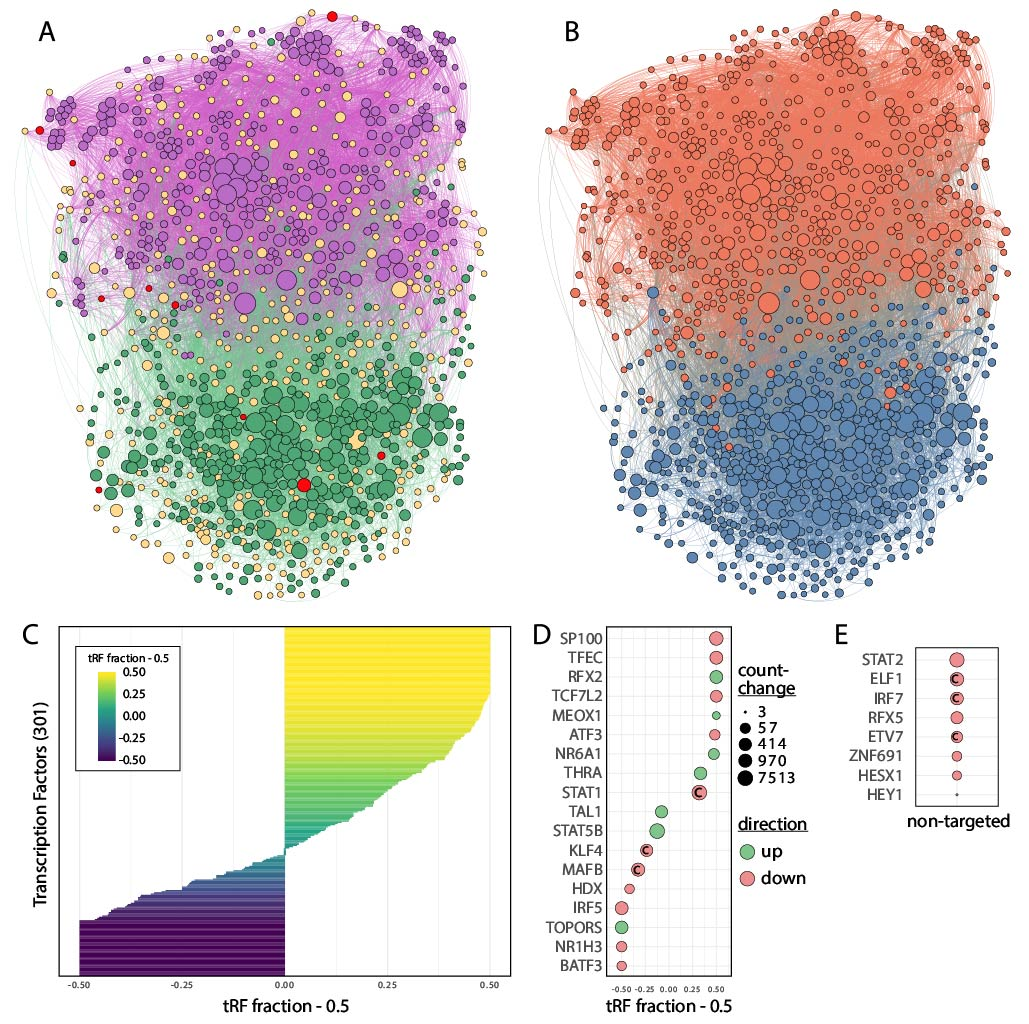
\includegraphics[width=\textwidth]{figures/smrna-tf-network-fractions}
\caption[Small RNA Targeting of Transcription Factors in CD14$^+$ Monocytes.]{\textbf{Small RNA Targeting of Transcription Factors in CD14$^+$ Monocytes.} The two-dimensional map of all TFs active in CD14$^+$ monocytes and their smRNA controllers was created via \emph{miRNeo} targeting and visualisation via force-directed algorithm. Node size is determined by activity (see Section \ref{sec:stroke:circuit-network}). \textbf{A)} Nodes coloured by biotype: miRNAs - green, tRFs - purple, TFs - yellow, differentially expressed (DE) TFs - red. TFs targeted mainly by tRFs segregate visually from TFs targeted mainly by miRNAs. Both sets contain DE TFs, indicating complementary function. \textbf{B)} The network was divided into two modules by network connectivity measures. Node colour denotes modularity class association. Network modularity largely reflects TF targeting of tRFs (orange) versus miRNAs (blue). \textbf{C)} Bar graph displays the fraction of smRNAs of each species targeting each of the TFs (on the y-axis, 301 TFs). A tRF fraction of 1 means all smRNAs targeting the TF are tRFs, 0 means all are miRNAs. Displayed on x axis is »tRF fraction - 0.5« to center on 50:50 targeting by both species. 48 TFs are solely targeted by miRNAs (leftmost) and 58 solely by tRFs (rightmost). \textbf{D)} Similarly, TFs differentially expressed in the blood of stroke victims show a distribution on the miRNA-tRF gradient. Point size denotes count-change, point colour denotes direction of change; a »C« denotes the TF as targeting cholinergic core and receptor genes. \textbf{E)} Notably, there is also a set of TFs that are supposedly not targeted by any smRNA present in CD14$^+$ cells.
\label{fig:smrna-tf-network-fractions}}
\end{figure}

The \emph{STAT} family of transcription factors is an interesting example in this analysis. The cholinergic/neurokine interface is facilitated by JAK/STAT signalling, in which neurokine receptors can activate the pathway through STAT1, STAT3, and STAT5A/B phosphorylation.\cite{Lobentanzer2019a} There are three differentially expressed STATs in our data set: STAT1 is down-regulated (highest absolute count-change of all TFs), targeted preferentially by tRFs (tRF fraction = 82.1\%), and directly associated with cholinergic genes in CD14$^+$ monocytes (»C«); STAT5B is up-regulated (second highest count-change of all TFs), preferentially targeted by miRNAs (tRF fraction = 37.5\%), and not directly associated with cholinergic genes in CD14$^+$ cells; and STAT2 is also down-regulated (third highest absolute count-change of all TFs), does not directly associate with cholinergic genes, and additionally is not predicted to be targeted by any smRNA present in CD14$^+$ monocytes, although it is expressed and induced by interferons in these cells.\cite{Lehtonen1997} 

\subsection{Dichotomous Transcriptomic Footprints of \\Transcription Factors in CD14$^+$ Monocytes}
To determine the putative effect of TF regulation by each smRNA species, we evaluated the potential impact of the TFs most targeted by either miRNAs or tRFs (i.e., the two modules from Figure \ref{fig:smrna-tf-network-fractions}\,B). The top 10\% of TF targets in CD14$^+$ monocytes (derived from Marbach \emph{et al.}\cite{Marbach2016}) were subjected to iterative GO analysis (see Section \ref{sec:stroke:go-cd14}). Assuming a general effect of repression in tRF-targeted TFs (because the majority of DE tRFs are up-regulated), and a general de-repression in the set of miRNA-targeted TFs (because most DE miRNAs are down-regulated), the putative functional effects of changes in smRNA levels can be described by GO enrichment analysis of these two test sets. Although this is a very rough categorisation, it may help in classifying the areas of influence shared between the two smRNA species, or exclusive to either.

\subsubsection{GO Term Overlap Between miRNA- and tRF-targeted \\Transcription Factors}
If we assume the functions associated with TF$\to$gene interaction (the »footprint«) in each subnetwork under miRNA or tRF control as an indication of the sphere of (most) influence of this smRNA species, the GO terms associated with both can give an indication of their overlapping functions. Further assuming the simplified scenario of dominating de-repression in miRNA-controlled transcripts, and dominating repression in tRF-controlled transcripts, this set of overlapping function is the set where a homeostasis is met by the cooperation of miRNAs and tRFs, or where, upon perturbations such as stroke, a shift in the balance between the two smRNA species can alter the physiological response to the stimulus.

We found 39 significant GO terms to overlap between multiple sets of miRNA- and tRF-targeted transcription factors, almost exclusively comprised of immunity-related terms. Seven terms were found with adjusted p-value < 0.001, namely: neutrophil chemotaxis (p = \me{1.3}{4}), regulation of myeloid leukocyte differentiation (\me{2.6}{4}), positive regulation of cold-induced thermogenesis (\me{2.8}{4}), negative regulation of ERK1 and ERK2 cascade (\me{3.0}{4}), regulation of type 2 immune response (\me{4.9}{4}), regulation of antigen receptor-mediated signalling pathway (\me{5.0}{4}), and negative regulation of IFN-$\upgamma$ production (\me{5.9}{4}). Further terms included positive regulation of CD4$^+$, alpha-beta T cell activation (p = 0.0013), monocyte chemotaxis (0.0018), negative regulation of immune response (0.0021), response to hypoxia (0.0041), positive regulation of cytokine secretion (0.0049), and parasympathetic nervous system development (0.0051).

\subsubsection{Functions Distinguishing Between miRNA- and tRF-targeted \\Transcription Factors}
After removal of the overlapping GO terms between miRNA- and tRF-targeted transcription factors, the remaining miRNA- and tRF-associated sets were examined to assess their differences. In the following, only terms which had been found in at least two steps of the five-step iterative process are considered. Terms found in both sets that were not identical but very similar were also removed from the analysis.

Transcription factors from the module targeted preferentially by miRNAs (Figure \ref{fig:smrna-tf-network-fractions}\,B, blue) are active towards genes that implicate the following biological processes; several terms showed adjusted p-values below 0.001: response to TNF (p = \me{1.2}{4}), erythrocyte differentiation (\me{2.6}{4}), cellular response to cytokine stimulus (\me{3.5}{4}), positive regulation of cytokine production (\me{3.8}{4}), positive regulation of myeloid cell differentiation (\me{3.9}{4}), regulation of IL-12 production (\me{4.9}{4}), positive regulation of leukocyte chemotaxis (\me{6.5}{4}), regulation of cellular response to insulin (\me{6.6}{4}), negative regulation of T cell mediated immunity (\me{8.1}{4}). Other terms include: regulation of macrophage activation (0.0021), response to LPS (0.0045), negative regulation of haematopoiesis (0.006), regulation of production of interleukins 1, 6, 12, 13, and 17 (all p < 0.005). These processes may, simply, be seen as amplified, since the general down-regulation of miRNAs would lead to a de-repression of their targets. However, in many cases of »regulation«, no direction is implied.

The processes regulated exclusively by miRNA-regulated TFs in this scenario thus are mainly related to pro-inflammatory events, more specifically, innate immune response, mediated by interferons and pro-inflammatory interleukins. An amplification of pro-inflammatory innate responses is contrasted by a reduction in haematopoiesis and T cell-mediated reactions.

Transcription factors from the module targeted preferentially by tRFs (Figure \ref{fig:smrna-tf-network-fractions}\,B, orange) are active towards genes that implicate the following processes; several terms showed adjusted p-values below 0.001: negative regulation of apoptotic process (\me{1.3}{4}), negative regulation of coagulation (\me{1.9}{4}), positive regulation of haematopoiesis (\me{1.9}{4}), regulation of IFN-$\upgamma$ production (\me{2.5}{4}), positive regulation of angiogenesis (\me{2.7}{4}), IL-4 production (\me{4.1}{4}), nuclear pore organisation (\me{4.5}{4}), monocyte differentiation (\me{5.0}{4}), leukocyte migration (\me{5.2}{4}), and T cell cytokine production (\me{6.4}{4}). Other terms include: negative regulation of NIK/NF-$\upkappa$B signalling (0.0016), macrophage differentiation (0.0030), lymphocyte activation involved in immune response (0.0032), negative regulation of leukocyte mediated immunity (0.0043), negative regulation of neuron death (0.0052), monocyte differentiation (0.0062), negative regulation of insulin receptor signalling pathway (0.013), natural killer cell activation (0.017), positive regulation of STAT cascade (0.019), sensory perception of pain (0.026), CD8$^+$, alpha-beta T cell activation (0.043), production of interleukins 2, 4, 6 (all p < 0.005). These processes, as opposed to the miRNA-associated processes, may be seen as attenuated, since a strong trend towards up-regulation is seen in tRFs; this again holds true only for terms where a direction is implicit or explicitly described.

The processes regulated exclusively by tRF-targeted TFs refer to apoptosis, coagulation, angiogenesis, myeloid leukocyte regulation, and interleukin/STAT signalling. Processes amplified via the putative de-repression include apoptosis, coagulation, NIK/NF-$\upkappa$B signalling, leukocyte activity and differentiation, and insulin-mediated signalling. Negatively impacted processes include haematopoiesis, angiogenesis, STAT signalling, and IL-2 production.

Immediately comparing miRNA- and tRF-associated processes, there are multiple functional overlaps even in the set curated to show only exclusive terms for either smRNA species. Specifically, the perturbations in both species seem to up-regulate innate immune response, particularly via INFs, TNF, interleukins, and myeloid leukocytes. Additionally, the perturbations in both species seem to have an additive suppressive effect on haematopoiesis and T cell activation.

\newpage
